\documentclass{beamer}

% xcolor and define colors -------------------------
\usepackage{xcolor}

% https://www.viget.com/articles/color-contrast/
\definecolor{purple}{HTML}{5601A4}
\definecolor{navy}{HTML}{0D3D56}
\definecolor{ruby}{HTML}{9a2515}
\definecolor{alice}{HTML}{107895}
\definecolor{daisy}{HTML}{EBC944}
\definecolor{coral}{HTML}{F26D21}
\definecolor{kelly}{HTML}{829356}
\definecolor{cranberry}{HTML}{E64173}
\definecolor{jet}{HTML}{131516}
\definecolor{asher}{HTML}{555F61}
\definecolor{slate}{HTML}{314F4F}

% Mixtape Sessions
\definecolor{picton-blue}{HTML}{00b7ff}
\definecolor{violet-red}{HTML}{ff3881}
\definecolor{sun}{HTML}{ffaf18}
\definecolor{electric-violet}{HTML}{871EFF}

\newcommand\pictonBlue[1]{{\color{picton-blue}#1}}
\newcommand\sun[1]{{\color{sun}#1}}
\newcommand\electricViolet[1]{{\color{electric-violet}#1}}
\newcommand\violetRed[1]{{\color{violet-red}#1}}

\newcommand\bgPictonBlue[1]{{\colorbox{picton-blue!20!white}{#1}}}
\newcommand\bgSun[1]{{\colorbox{sun!20!white}{#1}}}
\newcommand\bgElectricViolet[1]{{\colorbox{electric-violet!20!white}{#1}}}
\newcommand\bgVioletRed[1]{{\colorbox{violet-red!20!white}{#1}}}

\def\code#1{\texttt{#1}}

% Main theme colors
\definecolor{accent}{HTML}{00b7ff}
\definecolor{accent2}{HTML}{871EFF}
\definecolor{gray100}{HTML}{f3f4f6}
\definecolor{gray800}{HTML}{1F292D}


% Beamer Options -------------------------------------

% Background
\setbeamercolor{background canvas}{bg = white}

% Change text margins
\setbeamersize{text margin left = 15pt, text margin right = 15pt} 

% \alert
\setbeamercolor{alerted text}{fg = accent2}

% Frame title
\setbeamercolor{frametitle}{bg = white, fg = jet}
\setbeamercolor{framesubtitle}{bg = white, fg = accent}
\setbeamerfont{framesubtitle}{size = \small, shape = \itshape}

% Block
\setbeamercolor{block title}{fg = white, bg = accent2}
\setbeamercolor{block body}{fg = gray800, bg = gray100}

% Title page
\setbeamercolor{title}{fg = gray800}
\setbeamercolor{subtitle}{fg = accent}

%% Custom \maketitle and \titlepage
\setbeamertemplate{title page}
{
    %\begin{centering}
        \vspace{20mm}
        {\Large \usebeamerfont{title}\usebeamercolor[fg]{title}\inserttitle}\\
        {\large \itshape \usebeamerfont{subtitle}\usebeamercolor[fg]{subtitle}\insertsubtitle}\\ \vspace{10mm}
        {\insertauthor}\\
        {\color{asher}\small{\insertdate}}\\
    %\end{centering}
}

% Table of Contents
\setbeamercolor{section in toc}{fg = accent!70!jet}
\setbeamercolor{subsection in toc}{fg = jet}

% Button 
\setbeamercolor{button}{bg = accent}

% Remove navigation symbols
\setbeamertemplate{navigation symbols}{}

% Table and Figure captions
\setbeamercolor{caption}{fg=jet!70!white}
\setbeamercolor{caption name}{fg=jet}
\setbeamerfont{caption name}{shape = \itshape}

% Bullet points

%% Fix spacing between items
\let\olditemize=\itemize 
\let\endolditemize=\enditemize 
\renewenvironment{itemize}{\vspace{0.25em}\olditemize \itemsep0.25em}{\endolditemize}

%% Fix left-margins
\settowidth{\leftmargini}{\usebeamertemplate{itemize item}}
\addtolength{\leftmargini}{\labelsep}

%% enumerate item color
\setbeamercolor{enumerate item}{fg = accent}
\setbeamerfont{enumerate item}{size = \small}
\setbeamertemplate{enumerate item}{\insertenumlabel.}

%% itemize
\setbeamercolor{itemize item}{fg = accent!70!white}
\setbeamerfont{itemize item}{size = \small}
\setbeamertemplate{itemize item}[circle]

%% right arrow for subitems
\setbeamercolor{itemize subitem}{fg = accent!60!white}
\setbeamerfont{itemize subitem}{size = \small}
\setbeamertemplate{itemize subitem}{$\rightarrow$}

\setbeamertemplate{itemize subsubitem}[square]
\setbeamercolor{itemize subsubitem}{fg = jet}
\setbeamerfont{itemize subsubitem}{size = \small}








% Links ----------------------------------------------

\usepackage{hyperref}
\hypersetup{
  colorlinks = true,
  linkcolor = accent2,
  filecolor = accent2,
  urlcolor = accent2,
  citecolor = accent2,
}


% Line spacing --------------------------------------
\usepackage{setspace}
\setstretch{1.35}


% \begin{columns} -----------------------------------
\usepackage{multicol}


% Fonts ---------------------------------------------
% Beamer Option to use custom fonts
\usefonttheme{professionalfonts}

% \usepackage[utopia, smallerops, varg]{newtxmath}
% \usepackage{utopia}
\usepackage[sfdefault,light]{roboto}

% Small adjustments to text kerning
\usepackage{microtype}



% Remove annoying over-full box warnings -----------
\vfuzz2pt 
\hfuzz2pt


% Table of Contents with Sections
\setbeamerfont{myTOC}{series=\bfseries, size=\Large}
\AtBeginSection[]{
        \frame{
            \frametitle{Roadmap}
            \tableofcontents[current]   
        }
    }


% Tables -------------------------------------------
% Tables too big
% \begin{adjustbox}{width = 1.2\textwidth, center}
\usepackage{adjustbox}
\usepackage{array}
\usepackage{threeparttable, booktabs, adjustbox}
    
% Fix \input with tables
% \input fails when \\ is at end of external .tex file
\makeatletter
\let\input\@@input
\makeatother

% Tables too narrow
% \begin{tabularx}{\linewidth}{cols}
% col-types: X - center, L - left, R -right
% Relative scale: >{\hsize=.8\hsize}X/L/R
\usepackage{tabularx}
\newcolumntype{L}{>{\raggedright\arraybackslash}X}
\newcolumntype{R}{>{\raggedleft\arraybackslash}X}
\newcolumntype{C}{>{\centering\arraybackslash}X}

% Figures

% \imageframe{img_name} -----------------------------
% from https://github.com/mattjetwell/cousteau
\newcommand{\imageframe}[1]{%
    \begin{frame}[plain]
        \begin{tikzpicture}[remember picture, overlay]
            \node[at = (current page.center), xshift = 0cm] (cover) {%
                \includegraphics[keepaspectratio, width=\paperwidth, height=\paperheight]{#1}
            };
        \end{tikzpicture}
    \end{frame}%
}

% subfigures
\usepackage{subfigure}


% Highlight slide -----------------------------------
% \begin{transitionframe} Text \end{transitionframe}
% from paulgp's beamer tips
\newenvironment{transitionframe}{
    \setbeamercolor{background canvas}{bg=accent!40!black}
    \begin{frame}\color{accent!10!white}\LARGE\centering
}{
    \end{frame}
}


% Table Highlighting --------------------------------
% Create top-left and bottom-right markets in tabular cells with a unique matching id and these commands will outline those cells
\usepackage[beamer,customcolors]{hf-tikz}
\usetikzlibrary{calc}
\usetikzlibrary{fit,shapes.misc}

% To set the hypothesis highlighting boxes red.
\newcommand\marktopleft[1]{%
    \tikz[overlay,remember picture] 
        \node (marker-#1-a) at (0,1.5ex) {};%
}
\newcommand\markbottomright[1]{%
    \tikz[overlay,remember picture] 
        \node (marker-#1-b) at (0,0) {};%
    \tikz[accent!80!jet, ultra thick, overlay, remember picture, inner sep=4pt]
        \node[draw, rectangle, fit=(marker-#1-a.center) (marker-#1-b.center)] {};%
}


% DAGS ----------------------------------------------
\usepackage{tikz}
\usetikzlibrary{shapes,decorations,arrows,calc,arrows.meta,fit,positioning}
% Tikz settings optimized for causal graphs.
\tikzset{
    -Latex,auto,node distance =1 cm and 1 cm,semithick,
    state/.style ={ellipse, draw, minimum width = 0.7 cm},
    point/.style = {circle, draw, inner sep=0.04cm,fill,node contents={}},
    bidirected/.style={Latex-Latex,dashed},
    el/.style = {inner sep=2pt, align=left, sloped}
}


% Beamer tricks -------------------------------------
% Make \pause work in align environments
\makeatletter
\renewrobustcmd{\beamer@@pause}[1][]{%
  \unless\ifmeasuring@%
  \ifblank{#1}%
    {\stepcounter{beamerpauses}}%
    {\setcounter{beamerpauses}{#1}}%
  \onslide<\value{beamerpauses}->\relax%
  \fi%
}
\makeatother

\usepackage{breqn} % Breaks lines

\usepackage{amsmath}
\usepackage{mathtools}

\usepackage{pdfpages} % \includepdf

\usepackage{listings} % R code
\usepackage{verbatim} % verbatim

% Video stuff
\usepackage{media9}

% packages for bibs and cites
\usepackage{natbib}
\usepackage{har2nat}
\newcommand{\possessivecite}[1]{\citeauthor{#1}'s \citeyearpar{#1}}
\usepackage{breakcites}
\usepackage{alltt}

% Setup math operators
\DeclareMathOperator{\E}{E} \DeclareMathOperator{\tr}{tr} \DeclareMathOperator{\se}{se} \DeclareMathOperator{\I}{I} \DeclareMathOperator{\sign}{sign} \DeclareMathOperator{\supp}{supp} \DeclareMathOperator{\plim}{plim}
\DeclareMathOperator*{\dlim}{\mathnormal{d}\mkern2mu-lim}
\newcommand\independent{\protect\mathpalette{\protect\independenT}{\perp}}
   \def\independenT#1#2{\mathrel{\rlap{$#1#2$}\mkern2mu{#1#2}}}
\newcommand*\colvec[1]{\begin{pmatrix}#1\end{pmatrix}}

\newcommand{\myurlshort}[2]{\href{#1}{\textcolor{gray}{\textsf{#2}}}}


\begin{document}

\imageframe{./lecture_includes/mixtape_did_cover.png}


% ---- Content ----

\section{Background}

\subsection{Introduction}

\begin{frame}{Introduction}

\begin{itemize}
\item Welcome to a day long workshop on difference-in-differences 
\item Lecture, discussion, exercises, application using \url{https://github.com/Mixtape-Sessions/Causal-Inference-2/} as our homebase
\end{itemize}

\end{frame}

\begin{frame}{About Me}

\begin{itemize}
\item Scott Cunningham, Ben H. Williams Professor at Baylor University, Economist
\item Historical research is on sex work, drug policy, abortion policy
\item These days mental illness in corrections, suicidality, machine learning prediction and prevention
\item Author of \underline{Causal Inference: the Mixtape} and proprietor of ``Mixtape Sessions'', an online platform and offline workshop attempting to help link students and PhD researchers to emerging methods in causal inference
\end{itemize}

\end{frame}



\begin{frame}{NYU Workshop outline}

Part 1: Introduction to DiD basics 
	\begin{itemize}
	\item Potential outcomes review
	\item DiD equation and estimation with OLS
	\item Evaluating parallel trends with falsifications, event studies 
	\item Triple differences
	\end{itemize}

\end{frame}

\begin{frame}{NYU Workshop outline}

Part 2: Differential timing
	\begin{itemize}
	\item Fixed effects estimator and strict exogeneity
	\item Bacon decomposition of TWFE specification 
	\item Callaway and Sant'Anna solution
	\item Sun and Abraham solution to the event study
	\end{itemize}

\end{frame}

\begin{frame}{NYU Workshop outline}

Part 3: Synthetic Control 
	\begin{itemize}
	\item Abadie, et al. (2003; 2010) original synthetic control
	\item Ben-Michael, et al. (2021) augmented synthetic control
	\end{itemize}

\end{frame}




\begin{frame}{Natural experiments}

\begin{quote}
``A good way to do econometrics is to look for good natural experiments and use statistical methods that can tidy up the confounding factors that nature has not controlled for us.'' -- Daniel McFadden (Nobel Laureate recipient with Heckman 1992)
\end{quote}

\end{frame}


\imageframe{./lecture_includes/bumpersticker.jpeg}






\begin{frame}{What is difference-in-differences (DiD)}

\begin{itemize}
\item DiD is a very old, relatively straightforward, intuitive research design often used with ``natural experiment'' methodologies
\item One of the most widely used quasi-experimental methods in economics and even used in industry
\item Basic idea: a group of units receive some treatment and then compared to a group of units that do not
\end{itemize}

\end{frame}


\begin{frame}

	\begin{figure}
	\caption{Currie, et al. (2020)}
	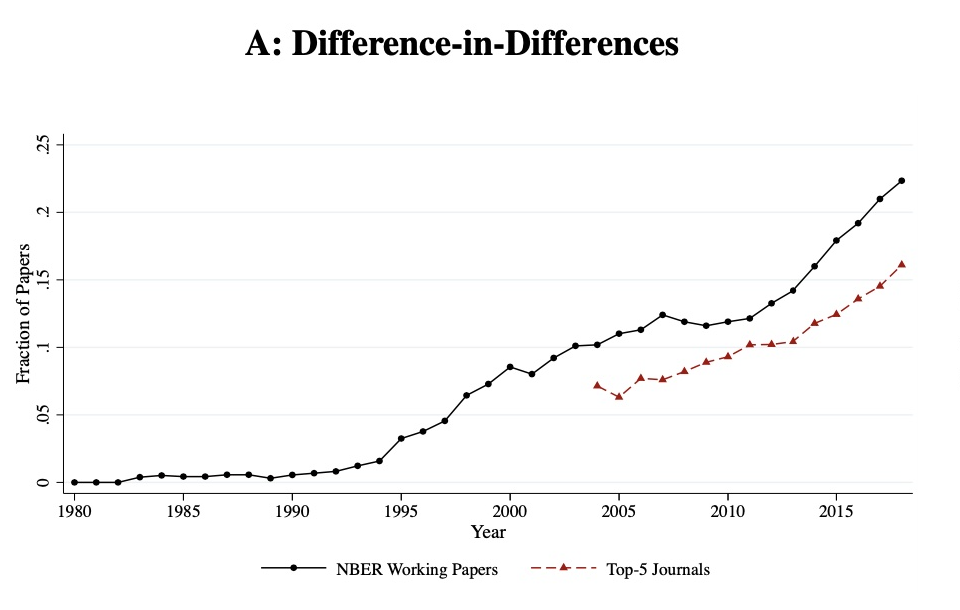
\includegraphics[scale=0.25]{./lecture_includes/currie_did.png}
	\end{figure}


\end{frame}








\begin{frame}{Origins in Economics and Public Health}

\begin{itemize}
\item In economics, David Card and Orley Ashenfelter are often associated with its origin -- used in the 1970s and 1980s, with mixed success, to study job training programs
\item Their dissatisfaction with it led to a call for more randomized controlled trials because, as we will see, it is not able to solve every kind of problem
\item But it predates economics by 150 years when two health scientists (separately) used it to prove disease transmission mechanisms

\end{itemize}

\end{frame}

\begin{frame}{Case I: Ignaz Semmelweis and washing hands}

\begin{itemize}
\item 1840s, Vienna maternity wards had high postpartum mortality in wings with doctors and trainee doctors, but not in wings with midwives and trainee midwives
\item Training hospitals of students had earlier moved to ``anatomical'' training involving cadavers for classes
\item Semmelweis thinks the mortality is caused by working with cadavers and proposes in 1847 physicians wash their hands with chlorine (but not midwives)
\item Comparing the two over time, he shows mortality in physician wing falls and concludes he was right (others disagree)
\end{itemize}

\end{frame}




\begin{frame}{Case II: John Snow and cholera}

\begin{itemize}
\item Three major waves of cholera in the early to mid 1800s in London and people mistakenly thought the cause was ``smelly air'' (or \emph{miasma})
\item John Snow argued that cholera was spread through host's evacuations, entering Thames river, returning through water supply
\item Strong evidence with maps and a novel DiD design: Lambeth water company moves its pipe between 1849 and 1854 but Southwark and Vauxhall delays
\end{itemize}

\end{frame}


\begin{frame}

	\begin{figure}
	\caption{Two water utility companies in London 1854}
	\includegraphics[scale=0.225]{./lecture_includes/lambeth.png}
	\end{figure}


\end{frame}


\begin{frame}{Three ways to study this}

\begin{enumerate}
\item Simple cross-section: compare mortality in 1854 for the two neighborhoods
\item Before and after: also called interrupted time series. Compare Lambeth in 1854 to 1849
\item Difference-in-differences: a combination of both
\end{enumerate}

\end{frame}



\begin{frame}{3) Difference-in-differences}

\begin{table}\centering
		\caption{Lambeth and Southwark and Vauxhall, 1849 and 1854}
		\begin{center}
		\begin{tabular}{lll|lc}
		\toprule
		\multicolumn{1}{l}{\textbf{Companies}}&
		\multicolumn{1}{c}{\textbf{Time}}&
		\multicolumn{1}{c}{\textbf{Outcome}}&
		\multicolumn{1}{c}{$D_1$}&
		\multicolumn{1}{c}{$D_2$}\\
		\midrule
		Lambeth & Before & $Y=L$ \\
		& After & $Y=L + \textcolor{red}{T_L} + \textcolor{blue}{D}$ & $\textcolor{red}{T_L}+\textcolor{blue}{D}$\\
		\midrule
		& & & & $\textcolor{blue}{D}$ \\
		\midrule
		Southwark and Vauxhall & Before & $Y=SV$ \\
		& After & $Y=SV + T_{SV}$ & $T_{SV}$\\
		\bottomrule
		\end{tabular}
		\end{center}
	\end{table}

\begin{eqnarray*}
\widehat{\delta}_{did} = \textcolor{blue}{D} + (\textcolor{red}{T_L} - T_{SV})
\end{eqnarray*}\textcolor{blue}{D} is the ``treatment effect''.  It's the effect of moving the water on Lambeth mortality and it's in blue because we can't see it 

\end{frame}

\begin{frame}{3) Difference-in-differences}

\begin{table}\centering
		\caption{Lambeth and Southwark and Vauxhall, 1849 and 1854}
		\begin{center}
		\begin{tabular}{lll|lc}
		\toprule
		\multicolumn{1}{l}{\textbf{Companies}}&
		\multicolumn{1}{c}{\textbf{Time}}&
		\multicolumn{1}{c}{\textbf{Outcome}}&
		\multicolumn{1}{c}{$D_1$}&
		\multicolumn{1}{c}{$D_2$}\\
		\midrule
		Lambeth & Before & $Y=L$ \\
		& After & $Y=L + \textcolor{red}{T_L} + \textcolor{blue}{D}$ & $\textcolor{red}{T_L}+\textcolor{blue}{D}$\\
		\midrule
		& & & & $\textcolor{blue}{D}$ \\
		\midrule
		Southwark and Vauxhall & Before & $Y=SV$ \\
		& After & $Y=SV + T_{SV}$ & $T_{SV}$\\
		\bottomrule
		\end{tabular}
		\end{center}
	\end{table}

\begin{eqnarray*}
\widehat{\delta}_{did} = \textcolor{blue}{D} + (\textcolor{red}{T_L} - T_{SV})
\end{eqnarray*}\textcolor{red}{$T_L$} is a natural change in mortality that would have happened had they not moved the pipe upstream.  It creates problems for us

\end{frame}



\begin{frame}{3) Difference-in-differences}

\begin{table}\centering
		\caption{Lambeth and Southwark and Vauxhall, 1849 and 1854}
		\begin{center}
		\begin{tabular}{lll|lc}
		\toprule
		\multicolumn{1}{l}{\textbf{Companies}}&
		\multicolumn{1}{c}{\textbf{Time}}&
		\multicolumn{1}{c}{\textbf{Outcome}}&
		\multicolumn{1}{c}{$D_1$}&
		\multicolumn{1}{c}{$D_2$}\\
		\midrule
		Lambeth & Before & $Y=L$ \\
		& After & $Y=L + \textcolor{red}{T_L} + \textcolor{blue}{D}$ & $\textcolor{red}{T_L}+\textcolor{blue}{D}$\\
		\midrule
		& & & & $D$ \\
		\midrule
		Southwark and Vauxhall & Before & $Y=SV$ \\
		& After & $Y=SV + T_{SV}$ & $T_{SV}$\\
		\bottomrule
		\end{tabular}
		\end{center}
	\end{table}

\begin{eqnarray*}
\widehat{\delta}_{did} = \textcolor{blue}{D} + (\textcolor{red}{T_L} - T_{SV})
\end{eqnarray*}But, if $\textcolor{red}{T_L}=\textcolor{black}{T_{SV}}$, which is called ``parallel trends'', then we can identify $\textcolor{blue}{D}$ using DiD.  And that's DiD in a nutshell. 

\end{frame}



\subsection{Potential outcomes}



\begin{frame}{Potential outcomes notation}

We need formal notation to understand DiD and that's the potential outcomes model

\bigskip
	
	\begin{itemize}
	\item Let the treatment be a binary variable: $$D_{i,t} =\begin{cases} 1 \text{ if pipe inlet is upstream at time $t$} \\ 0 \text{ if pipe inlet is downstream at time $t$} \end{cases}$$where $i$ indexes an individual observation, such as a person

	\end{itemize}
\end{frame}

\begin{frame}{Potential outcomes notation}
	
	\begin{itemize}

	\item Potential outcomes: $$Y_{i,t}^j =\begin{cases} 1 \text{: health if drank from upstream at time $t$} \\ 0 \text{: health if drank from downstream at time $t$} \end{cases}$$where $j$ indexes a counterfactual state of the world

	\end{itemize}
\end{frame}


\begin{frame}{Potential vs realized}

\begin{itemize}
\item Data are ``realized outcomes'' not ``potential outcomes''
\item Realized outcomes is ``selected'' when treatments are assigned: $$Y_{it}=D_{it}Y_{it}^1 + (1-D_{it})Y_{it}^0$$
\item Example: My wages if I go to college are $Y^1$ and my wages if I don't go to college are $Y^0$, but since I went to college ($D=1$), my wages are $Y=Y^1$.

\end{itemize}
\end{frame}



\begin{frame}{Treatment effect definitions}


	\begin{block}{Individual treatment effect}
	    The individual treatment effect,  $\delta_i$, equals $Y_i^1-Y_i^0$
	\end{block}

Core building block of causal inference is the individual treatment effect. 
	
\end{frame}



\begin{frame}{Conditional Average Treatment Effects}	
	\begin{block}{Average Treatment Effect on the Treated (ATT)}
	The average treatment effect on the treatment group is equal to the average treatment effect conditional on being a treatment group member:
		\begin{eqnarray*}
		E[\delta|D=1]&=&E[Y^1-Y^0|D=1] \nonumber \\
		&=&E[Y^1|D=1]-\textcolor{red}{E[Y^0|D=1]} \\
		&=&E[Y|D=1]-\textcolor{red}{E[Y^0|D=1]}
		\end{eqnarray*}
	\end{block}
	
	\bigskip
	
We have $E[Y^1|D=1]$ but we don't have \textcolor{red}{$E[Y^0|D=1]$} so DiD imputes it using something called ``parallel trends'' (a strong assumption)

	
\end{frame}

\section{Identification and Estimation}

\subsection{Parallel trends}


\begin{frame}{Steps of your causal projects}

\begin{enumerate}
\item Define the parameter we want (``ATT''), 
\item Ask what what beliefs do you need (``identification''), and 
\item Build cranks that produce the correct numbers (``estimator'')
\end{enumerate}

\bigskip

People often skip 1 and 2 and go straight to 3 and run regressions then go back and assume exogeneity (step 2), and hope that the estimates are weighted averages of individual treatment effects (1), but that is not guaranteed

\bigskip

Assume we are interested in the ATT.  What must be true for which method to estimate it correctly?

\end{frame}



\begin{frame}{DiD is four averages and three differences}

Let $k$ and $U$ index the treatment (Lambeth) and untreated group (Southwark and Vauxhall)

\begin{eqnarray*}
\widehat{\delta}^{2x2}_{kU} = \bigg ( E[Y_k|Post] - E[Y_k|Pre] \bigg ) - \bigg ( E[Y_U | Post ] - E[ Y_U | Pre] \bigg) \\
\end{eqnarray*}

\bigskip

``Pre'' (1849) and ``Post'' (1854) refer to when Lambeth, $k$, was treated which is why it is the same for both $k$ and $U$ groups


\end{frame}



\begin{frame}{Potential outcomes and the switching equation}

From DiD to ATT

\begin{eqnarray*}
\widehat{\delta}^{2x2}_{kU} &=&  \bigg ( \underbrace{E[Y_k|Post] - E[Y_k|Pre] \bigg ) - \bigg ( E[Y_U | Post ] - E[ Y_U | Pre]}_{\mathclap{\text{DiD equation}}} \bigg)  \\
&=& \bigg ( \underbrace{E[Y^1_k|Post] - E[Y^0_k|Pre] \bigg ) - \bigg ( E[Y^0_U | Post ] - E[ Y^0_U | Pre]}_{\mathclap{\text{Replace with potential outcomes using switching equation}}} \bigg)  \\
&&+ \underbrace{\textcolor{red}{E[Y_k^0 |Post] - E[Y^0_k | Post]}}_{\mathclap{\text{Plus zero}}} 
\end{eqnarray*}

\end{frame}

\begin{frame}{Parallel trends bias}

Rearrange and we get this:

\begin{eqnarray*}
\widehat{\delta}^{2x2}_{kU} &=& \underbrace{E[Y^1_k | Post] - \textcolor{red}{E[Y^0_k | Post]}}_{\mathclap{\text{ATT}}} \\
&& + \bigg [  \underbrace{\textcolor{red}{E[Y^0_k | Post]} - E[Y^0_k | Pre] \bigg ] - \bigg [ E[Y^0_U | Post] - E[Y_U^0 | Pre] }_{\mathclap{\text{Non-parallel trends bias}}} \bigg ]
\end{eqnarray*}

\bigskip

The left hand side is our DiD estimator (i..e, four averages, three differences); the right hand side has our parameter (top) and assumption (parallel trends, bottom).  

\bigskip

Recall from the earlier table how DiD was equal to $D+(\textcolor{red}{T_L} - T_{SV})$.  That's this.



\end{frame}



\begin{frame}{Identification through parallel trends}
	

	\begin{block}{Parallel trends}
	Assume two groups, treated and comparison group, then we define parallel trends as:	 $$\textcolor{red}{E(}\textcolor{red}{\Delta Y^0_k)} = E(\Delta Y^0_U)$$
	\end{block}

\textbf{In words}: ``The \textcolor{red}{evolution of cholera mortality for Lambeth \emph{had it kept its pipe downstream}} is the same as the evolution of cholera mortality for Southwark and Vauxhall''.  

\bigskip

It's in \textcolor{red}{red} so you know it's a nontrivial assumption.  But why?  Can't we just check?

	

	
\end{frame}


\begin{frame}{Homework}

\begin{itemize}
\item I've included a simple exercise to really pin down these core ideas with simple calculations
\item Please at your leisure work through this exercise
\end{itemize}

\bigskip 

\url{https://docs.google.com/spreadsheets/d/1onabpc14JdrGo6NFv0zCWo-nuWDLLV2L1qNogDT9SBw/edit?usp=sharing}

\end{frame}



\subsection{Estimation with OLS specification}

\begin{frame}{OLS Specification}
	
	\begin{itemize}
	\item Simple DiD equation (four averages, three differences) estimates ATT under parallel trends; don't need regression
	\item But there is an OLS specification that is numerically identical to four averages and three differences
	\item OLS was historically preferred because
		\begin{itemize}
		\item OLS estimates the ATT under parallel trends so it is valid
		\item Easy to calculate the standard errors
		\item Easy to include multiple periods which increases power and makes estimates more precise
		\end{itemize}
	\item This specification is not appropriate under differential timing or with the inclusion of covariates
	\end{itemize}
\end{frame}

\begin{frame}{Minimum wages}

\begin{itemize}
\item Card and Krueger (1994) have a famous study estimating causal effect (ATT) of minimum wages on employment
\item Exploited a policy change in New Jersey between February and November in mid-1990s where minimum wage was increased, but neighbor PA did not
\item Using DiD, they do not find a negative effect of the minimum wage on employment which is part of its legacy today, but I mainly present it to illustrate the history and the design principles
\end{itemize}

\end{frame}

\begin{frame}
	\begin{figure}
	
\includegraphics[scale=0.5]{./lecture_includes/minwage_whore}
	\end{figure}
\end{frame}

\begin{frame}{Quick comment}

\begin{itemize}
\item Buchanan's comment gets taken out of historical context to a degree
\item Empirical labor and empirical macroeconomics (e.g., Lucas Critique) had been going back to the 1970s in a bit of a ``empirical crisis'' much like we see sometimes today with debates about p-hacking, but theirs was more basic confusion of causality and correlation
\item Consequently, the dominant paradigm in ``knowing facts in economics'' was theory, not empiricism
\item So Buchanan's dismissiveness probably had traces of that; quality of empirical work was sub standard so people tended to not take it very seriously
\end{itemize}

\end{frame}


\begin{frame}{Card on that study}

\begin{quote}
``I’ve subsequently stayed away from the minimum wage literature for a number of reasons. First, it cost me a lot of friends. People that I had known for many years, for instance, some of the ones I met at my first job at the University of Chicago, became very angry or disappointed. They thought that in publishing our work we were being traitors to the cause of economics as a whole.''
\end{quote}

\bigskip

But let's listen to Orley's opinion about the paper's controversy at the time.  \url{https://youtu.be/bbW62axQum8}

\end{frame}



\begin{frame}{OLS specification of the DiD equation}
	
	\begin{itemize}
	\item The correctly specified OLS regression is an interaction with time and group fixed effects:$$Y_{its} = \alpha + \gamma NJ_s + \lambda d_t + \delta (NJ \times d)_{st} + \varepsilon_{its}$$
		\begin{itemize}
		\item NJ is a dummy equal to 1 if the observation is from NJ
		\item d is a dummy equal to 1 if the observation is from November (the post period)
		\end{itemize}
	\item This equation takes the following values
		\begin{itemize}
		\item PA Pre: $\alpha$
		\item PA Post: $\alpha + \lambda$
		\item NJ Pre: $\alpha + \gamma$
		\item NJ Post: $\alpha + \gamma + \lambda + \delta$
		\end{itemize}
	\item DiD equation: (NJ Post - NJ Pre) - (PA Post - PA Pre) $= \delta$
	\end{itemize}
\end{frame}




\begin{frame}[plain]
	$$Y_{ist} = \alpha + \gamma NJ_s + \lambda d_t + \delta(NJ\times d)_{st} + \varepsilon_{ist}$$
	\begin{figure}
	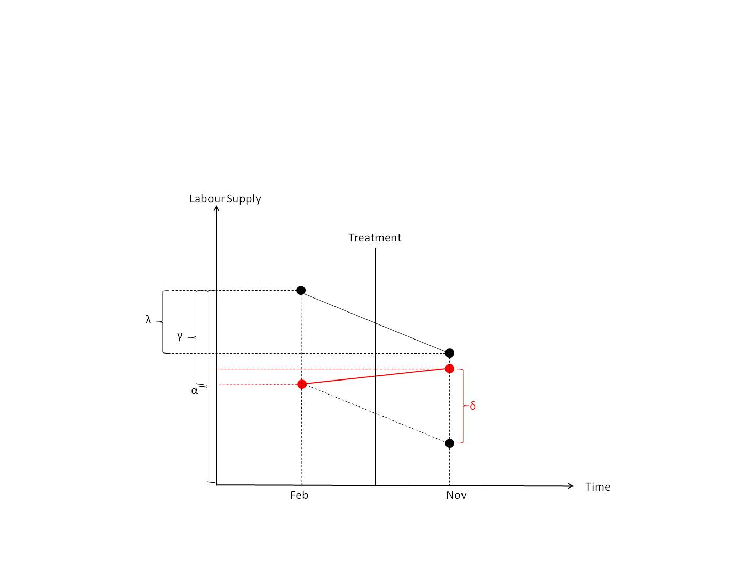
\includegraphics[scale=0.90]{./lecture_includes/waldinger_dd_5.pdf}
	\end{figure}
\end{frame}


\begin{frame}[plain]
	$$Y_{ist} = \alpha + \gamma NJ_s + \lambda d_t + \delta(NJ\times d)_{st} + \varepsilon_{ist}$$
	\begin{figure}
	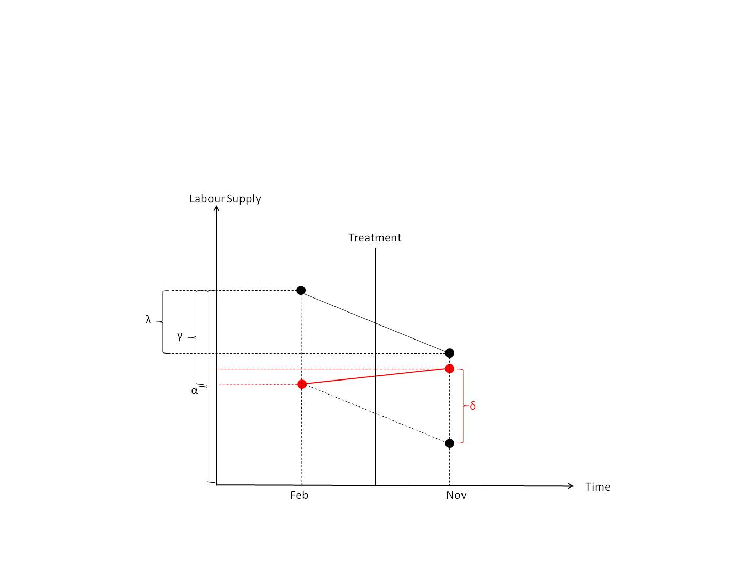
\includegraphics[scale=0.90]{./lecture_includes/waldinger_dd_5.pdf}
	\end{figure}

Notice how OLS is ``imputing'' $E[Y^0|D=1,Post]$ for the treatment group in the post period? It is only ``correct'', though, if parallel trends is a good approximation

\end{frame}

\subsection{Inference}

\begin{frame}{Inference}
	
	\begin{itemize}
	\item  Bertrand, Duflo and Mullainathan (2004) show that conventional standard errors will often severely understate the standard deviation of the estimators
	\item Standard errors are biased downward (i.e., too small, over reject)
	\item They proposed three solutions, but most only use one of them (clustering)
	\end{itemize}
\end{frame}


\begin{frame}{Inference}
	
		\begin{enumerate}
		\item[1 ] Block bootstrapping standard errors (if you analyze states the block should be the states and you would sample whole states with replacement for bootstrapping)
		\item[2 ] Clustering standard errors at the group level (in Stata one would simply add \texttt{, cluster(state)} to the regression equation if one analyzes state level variation)
		\end{enumerate}

\bigskip

Most people will simply cluster, but there are issues if you have too few clusters. They mention a third way but it's only a curiosity.
		
\end{frame}




\section{Parallel trends violations}

\subsection{How parallel trends can get violated}


\begin{frame}{Violating parallel trends exercise}

\begin{itemize}
\item Parallel trends guides the regression's hand to correctly impute counterfactual \textcolor{red}{$E[Y^0|D=1]$} using $\Delta E[Y^0|D=0]$ 
\item OLS \emph{always} imputes using $\Delta E[Y^0|D=0]$ but is only valid under parallel trends which means control groups matter
\item To illustrate this, I've included a document (tab is ``DID 2'') for you to work on at your leisure
\end{itemize}

\url{https://docs.google.com/spreadsheets/d/1onabpc14JdrGo6NFv0zCWo-nuWDLLV2L1qNogDT9SBw/edit?usp=sharing}

\end{frame}






\subsection{Types of evidence}

\begin{frame}{Think like a prosecutor}

\begin{itemize}
\item You are a prosecutor building a case before a judge and jury battling the expert defense attorney and their witnesses -- what should evidence look like?
\item Some example of commonly used forms of evidence can help you
\item Common evidence mixes careful and informed logic about main results and mechanisms with falsifications and data visualization, primarily with the event study
\end{itemize}

\end{frame}

\begin{frame}{Five types of evidence}

\begin{enumerate}
\item \textbf{Bite}: Show that the treatment impacted first order behavior before showing how it affected second order behavior
\item \textbf{Main Results}: Show the primary outcome that your project is about
\item \textcolor{red}{\textbf{Mechanisms}}: Can you provide evidence of a plausible pathway by which the treatment moves from first order to second order outcomes?
\item \textbf{Event studies}: A particular kind of data visualization focused on pre- and post-treatment DiD coefficients in a regression equation
\item \textbf{Placebos}: Ruling out reasonable competing theories using the same regression model on different outcomes; can include triple differences
\end{enumerate}

\end{frame}


\begin{frame}{Event studies are mandatory}

	\begin{figure}
	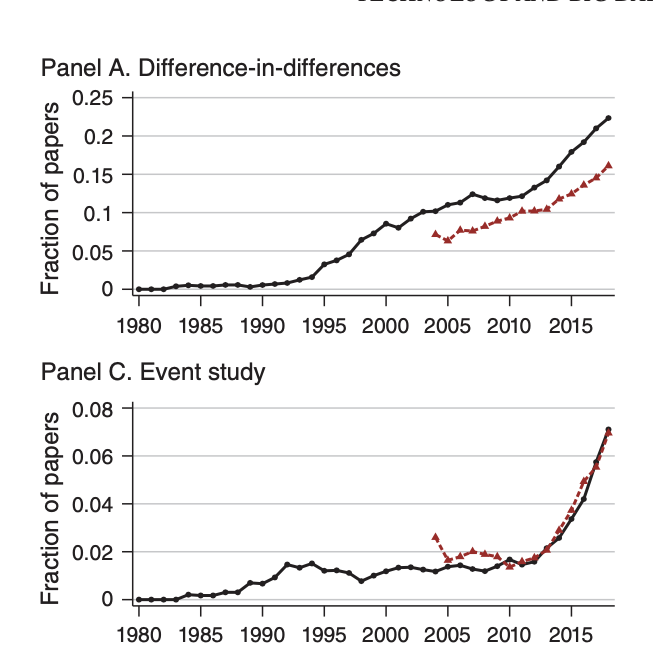
\includegraphics[scale=0.5]{./lecture_includes/currie_eventstudy.png}
	\end{figure}

\end{frame}

\begin{frame}{Intuition behind event studies}

\begin{itemize}
	\item We cannot verify parallel trends, but we can verify parallel \emph{pre-trends} 
	\item Pre-trends are a type of falsification -- there should not be any effect of the treatment before the treatment occurred
	\item Also provides some evidence that your comparison group may satisfy parallel trends since it satisfied it earlier
	\item Even if pre-trends are the same one still has to worry about other policies changing at the same time (omitted variable bias is a parallel trends violation)

\end{itemize}

\end{frame}




\begin{frame}{Plot the raw data when there's only two groups}

	\begin{figure}
	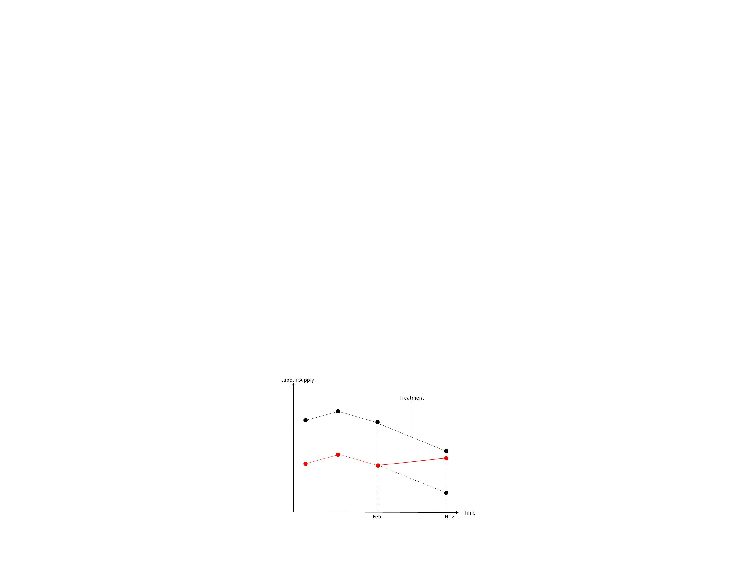
\includegraphics[scale=2.5]{./lecture_includes/waldinger_dd_6.pdf}
	\end{figure}

\end{frame}



\begin{frame}{Event study regression}
	
	\begin{itemize}
	\item Event studies have a simple OLS specification with only one treatment group and one never-treated group $$Y_{its} = \alpha +  \sum_{\tau=-2}^{-q}\mu_{\tau}D_{s\tau} + \sum_{\tau=0}^m\delta_{\tau}D_{s\tau}+\varepsilon_{ist}$$
		\begin{itemize}
		\item where $D$ is an interaction of the treatment group $s$ with the calendar year $\tau$
		\item Treatment occurs in year 0, no anticipation, drop baseline $t-1$
		\item Includes $q$ leads or anticipatory effects and $m$ lags or post treatment effects
		\end{itemize}
	\item But each OLS estimate of $\mu_\tau$ and $\delta_\tau$ are just ``four averages and three differences'' as that's the form of the saturated regression
	\end{itemize}
\end{frame}

\begin{frame}{Event study regression}


$$Y_{its} = \alpha + \sum_{\tau=-2}^{-q}\mu_{\tau}D_{s\tau} + \sum_{\tau=0}^m\delta_{\tau}D_{s\tau}+\varepsilon_{ist}$$

\bigskip

Typically you'll plot the coefficients and 95\% CI on all leads and lags (binned or not, trimmed or not) 

\bigskip

Under no anticipation, then you expect $\widehat{\mu}$ coefficients to be zero, which gives you confidence that parallel trends holds (but is not a guarantee, and there are still specification issues -- see Jon Roth's work)

\bigskip

Under parallel trends, $\widehat{\delta}$ are estimates of the ATT at points in time

\end{frame}



\begin{frame}{Medicaid and Affordable Care Act example}

\begin{figure}
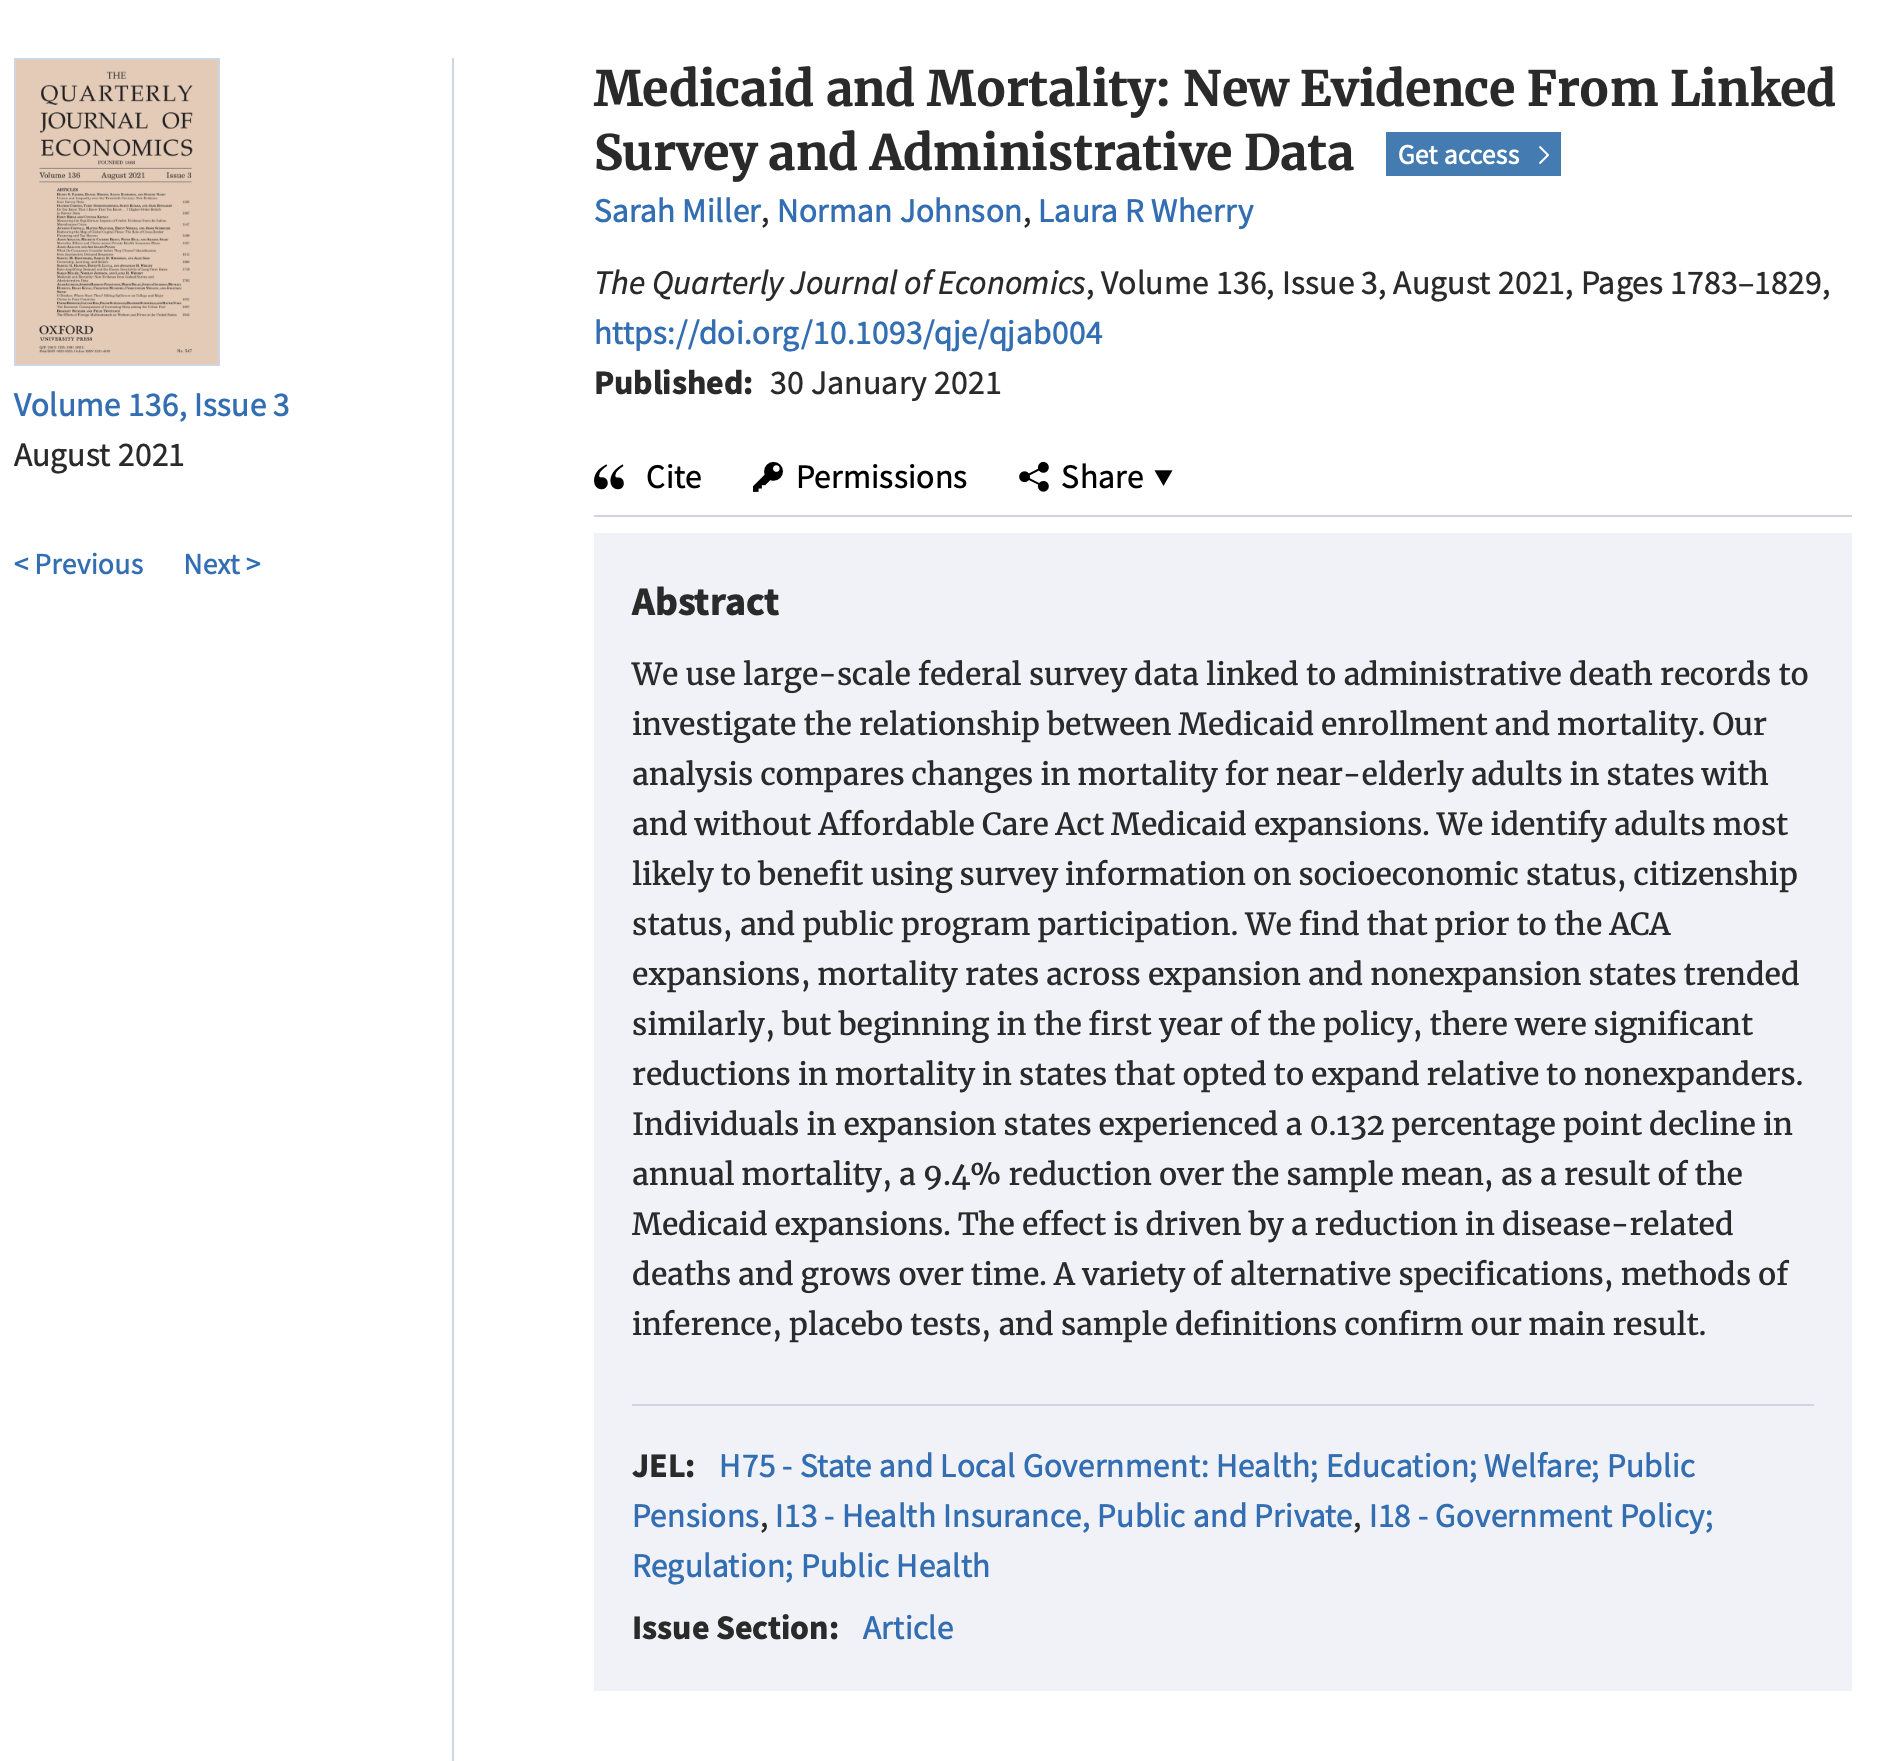
\includegraphics[scale=0.25]{./lecture_includes/medicaid_qje}
\end{figure}

\end{frame}

\begin{frame}{Their five types of evidence}

\begin{itemize}
\item \textbf{Bite} -- show that the expansion shifted people into Medicaid and out of uninsured status
\item \textbf{Main results} -- show that Medicaid expansion caused near-elderly mortality to fall 0.132pp or 9.4\% reduction from sample mean
\item \textcolor{red}{\textbf{Mechanism}} -- They suggest this is coming from reduced disease-related deaths which grows over time
\item \textbf{Placebos} -- Show that there's no effect on mortality for groups it shouldn't be affecting (people 65+)
\item \textbf{Event study} -- Show leads and lags on mortality
\end{itemize}

\end{frame}


\imageframe{./lecture_includes/Miller_Medicaid1.png}

\imageframe{./lecture_includes/Miller_Medicaid2.png}

\imageframe{./lecture_includes/Miller_Medicaid3.png}

\begin{frame}{Quick review}

\begin{itemize}

\item \textbf{Bite}: Did the expansion of Medicaid put more people on Medicaid?
	\begin{enumerate}
	\item 40pp increase in people eligible (but this was mechanical)
	\item 6-10pp increase in people on Medicaid (but maybe it was crowding out private insurance?)
	\item 4-6pp decrease in uninsured (at least some of the marginal Medicaid enrollees had been uninsured)
	\end{enumerate}
\end{itemize}

\end{frame}


\begin{frame}{65 and older mortality placebo}

	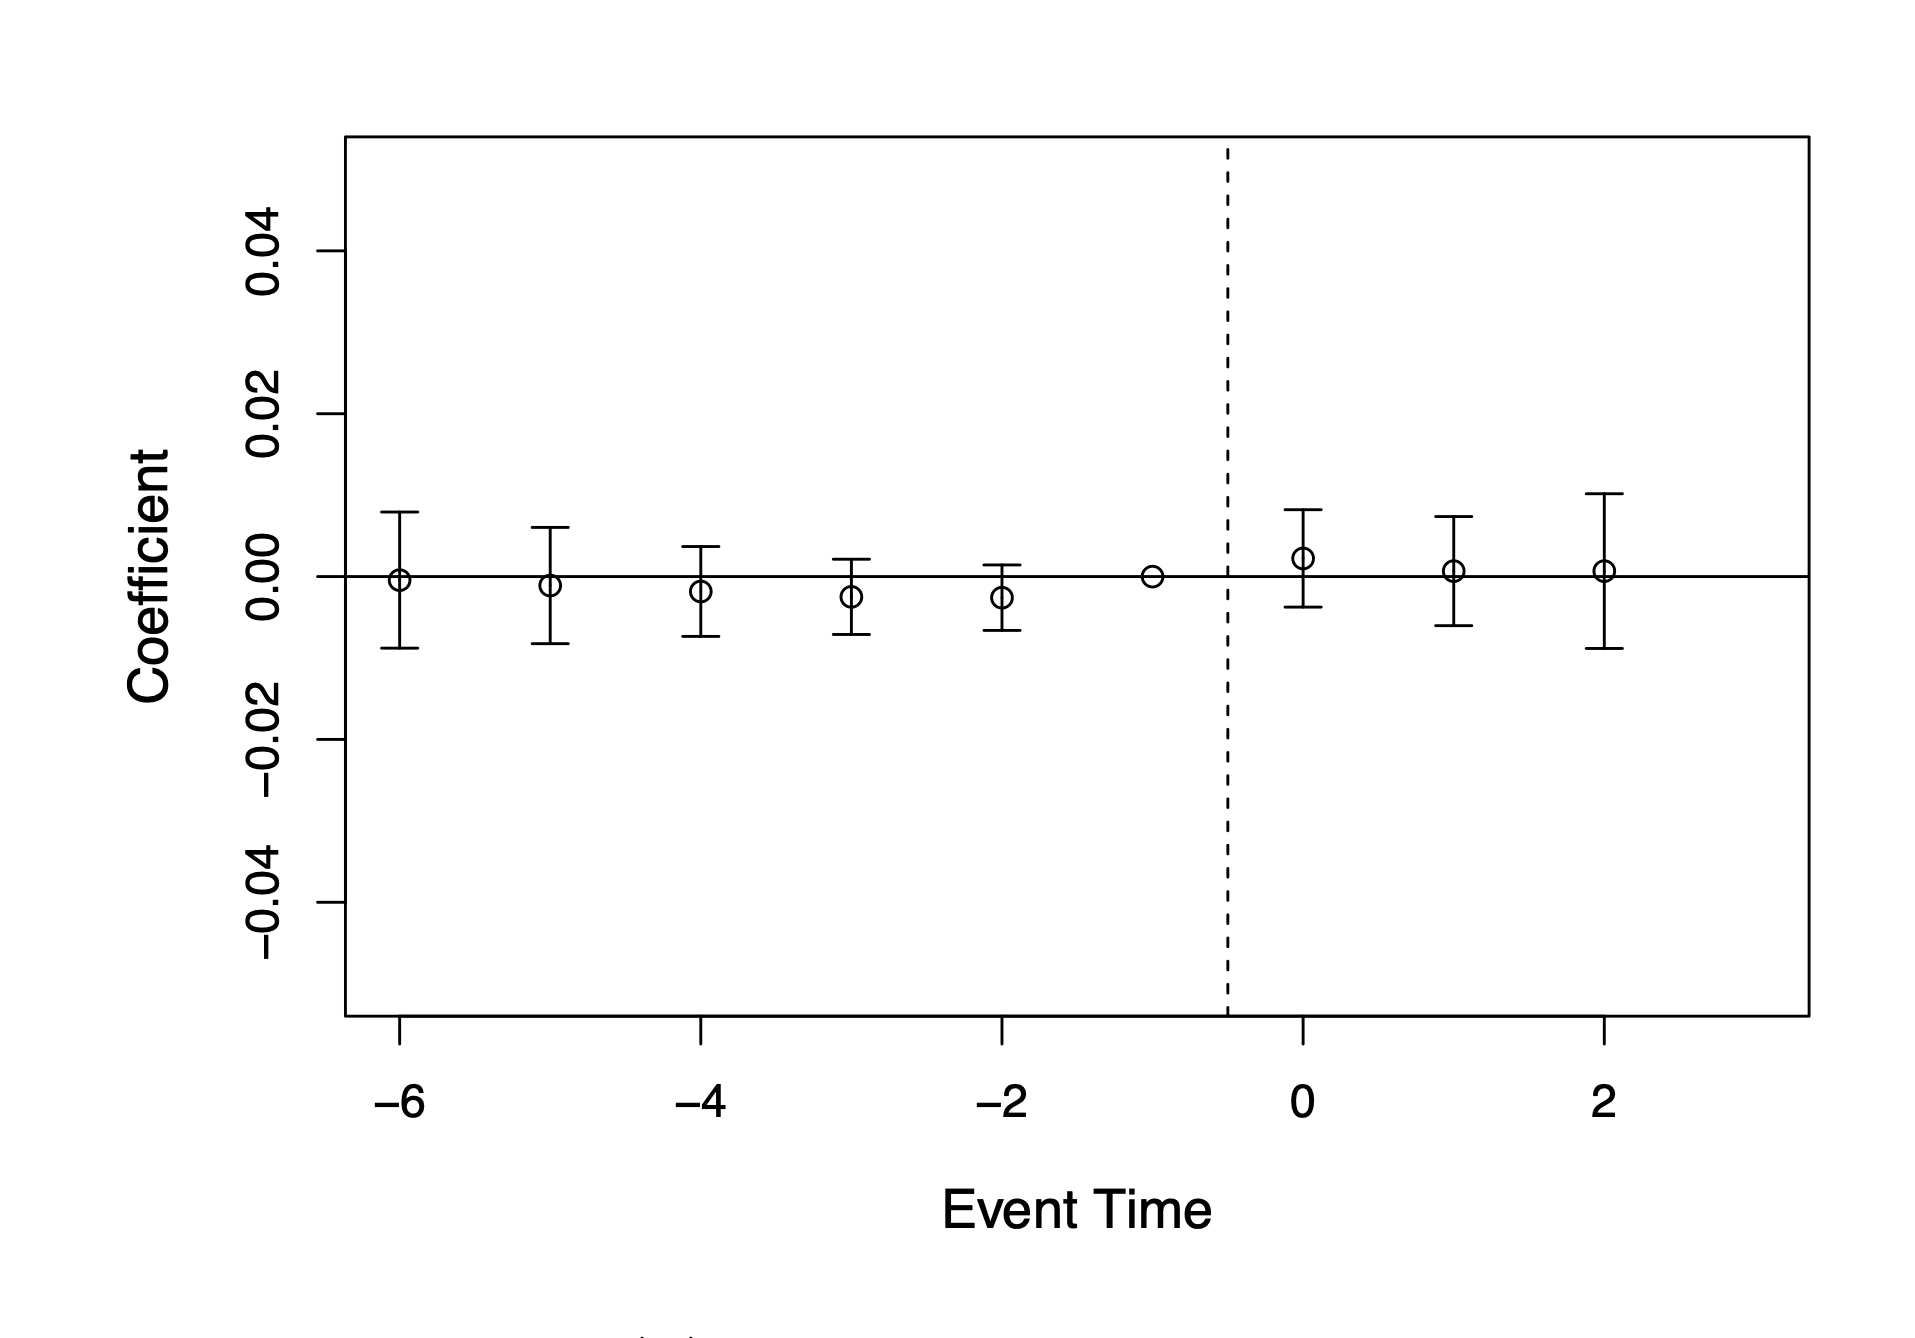
\includegraphics[scale=0.3]{./lecture_includes/medicaid_qje_placebo}

\textbf{Discussion}: Why do they do this?  Explain to me like I'm 5 the value of a picture like this.

\end{frame}
\begin{frame}{Main Results: Medicaid expansion and near-elderly mortality}

	\begin{figure}
	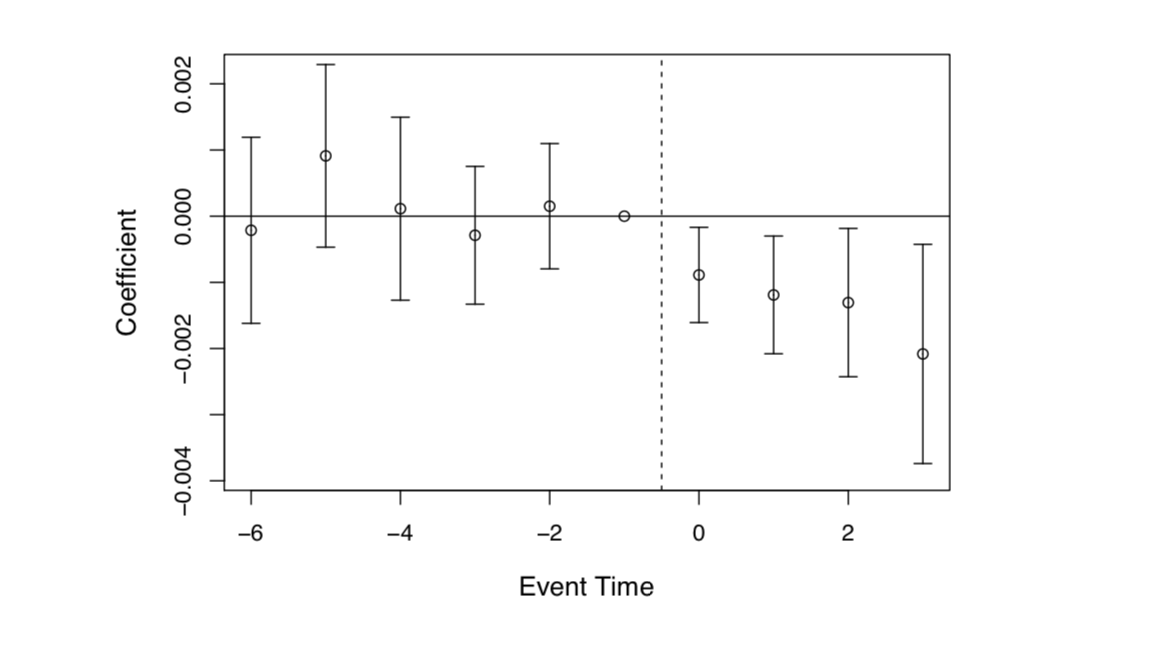
\includegraphics[scale=0.3]{./lecture_includes/Miller_Medicaid4.png}
	\end{figure}

\end{frame}

\begin{frame}{Lab}

\begin{itemize}

\item I've provided a lab for you to deepen your understanding of the simple mechanics involved in estimating DiD and event studies
\item Please go to this link \url{https://github.com/Mixtape-Sessions/Causal-Inference-2/tree/main/Lab/Lalonde}
\item Q1:a-c vs. Q2a.  Skip the covariates

\end{itemize}

\end{frame}

\subsection{Triple difference}

\begin{frame}{Triple differences as alternative strategy}
	
	\begin{itemize}
	\item Very common for readers and others to request a variety of ``robustness checks'' from a DD design
	\item We saw some of these just now (e.g., falsification test using data for alternative control group, the Medicare population)
	\item Triple differences uses a within-state untreated group; little trickier, so let's use the table again
	\end{itemize}
\end{frame}

\begin{frame}{DDD Example by Gruber}
	
	\begin{figure}
	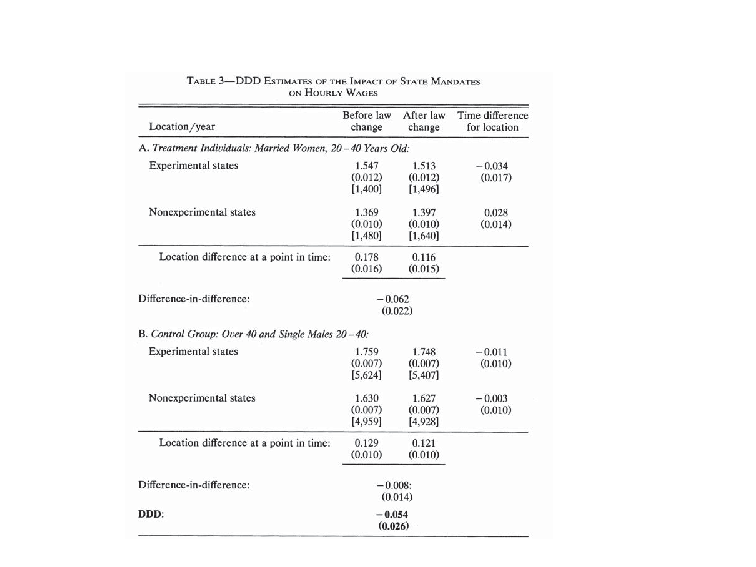
\includegraphics{./lecture_includes/gruber_ddd_3.pdf}
	\end{figure}
	
\end{frame}



\begin{frame}[shrink=20]

\begin{table}\centering
		\caption{Difference-in-Difference-in-Differences numerical example}
		\tiny
		\begin{center}
		\begin{tabular}{lll|l|lll}
		\hline \hline
		\multicolumn{1}{l}{\textbf{States}}&
		\multicolumn{1}{c}{\textbf{Group}}&
		\multicolumn{1}{c}{\textbf{Period}}&
		\multicolumn{1}{c}{\textbf{Outcomes}}&
		\multicolumn{1}{c}{$D_1$}&
		\multicolumn{1}{c}{$D_2$}&
		\multicolumn{1}{c}{$D_3$}\\
		\hline
		&&After	&$NJ+T+NJ_t+l_t+D$					\\
	&Married women, 20-40yo			&&&$T+NJ_t+l_t+D$			\\
		&&Before	&$NJ$					\\
Experimental states					&&&&&$D+\textcolor{red}{l_t-s_t}$			\\
		&&After	&$NJ+T+NJ_t+s_t$					\\
	&Older 40, Single men 20-40yo		&&	&$T+NJ_t+s_t$				\\
		&&Before	&$NJ$					\\
								\\
&&&&&&$D$
\\
		&&After	&$PA+T+PA_t+l_t$				\\
	&Married women, 20-40yo			&&&$T+PA_t+l_t$ \\				
		&&Before	&$PA$					\\
Non-experimental states					&&&&&$l_t-s_t$		\\
		&&After	&$PA+T+PA_t+s_t$					\\
	&Older 40, Single men 20-40yo		&&&	$T+PA_t+s_t$				\\
		&&Before	&$PA$					\\
		\hline \hline
		\end{tabular}
		\end{center}
	\end{table}
	
\textbf{What is our identifying assumption?} 

\bigskip

\textbf{Answer:} $\textcolor{red}{l_t-s_t}$ is the same for both experimental and non-experimental states. This is ``change in inequality between two groups hourly wages'' from pre to post.  It's a new parallel trend assumption.



\end{frame}


\begin{frame}{DDD in Regression}
	
	\begin{eqnarray*}
	Y_{ijt} &=&\alpha +  \beta_2 \tau_t + \beta_3 \delta_j  + \beta_4 D_i + \beta_5(\delta \times \tau)_{jt} \\
	&& +\ \beta_6(\tau \times D)_{ti} +  \beta_7(\delta \times D)_{ij} +  \textcolor{red}{\beta_8(\delta \times \tau \times  D)_{ijt}}+  \varepsilon_{ijt}
	\end{eqnarray*}
	
	\begin{itemize}
	\item Your panel is now a group $j$ state $i$ (e.g., AR high wage worker 1991, AR high wage worker 1992, etc.)
	\item Assume we drop $\tau_t$ but I just want to show it to you for now.
	\item If the placebo DD is non-zero, it might be difficult to convince the reviewer that the DDD removed all the bias 
	\end{itemize}
	
\end{frame}




\begin{frame}{Concluding remarks}

\begin{itemize}
\item So we hopefully see a few of the key elements of DiD
	\begin{itemize}
	\item Remember: the DiD equation and ATT equation are distinct concepts and definitions
	\item DiD designs can be implemented with OLS specifications that calculate differences in means
	\item Parallel pre-trends and parallel trends are not the same thing -- the first is testable, the latter is not testable
	\item Event studies are mandatory but pre-trends are smoking guns, but can mislead nonetheless
	\end{itemize}
\item Now we want to move into the fixed effects work
\end{itemize}

\end{frame}



\end{document}
